\documentclass[a4paper, 12pt]{extarticle}
\usepackage[dvipsnames]{xcolor}
\usepackage[top=70pt,bottom=70pt,left=48pt,right=46pt]{geometry}
\definecolor{header}{RGB}{252, 171, 16}
\definecolor{defenition}{RGB}{248, 51, 60}
\definecolor{main_title}{RGB}{43, 158, 179}
\definecolor{sub_header}{RGB}{68, 175, 105}
\usepackage[english, russian]{babel}
\usepackage[utf8]{inputenc}
\usepackage{amsmath}
\usepackage[most]{tcolorbox}
\usepackage{listings}
\usepackage{graphicx}
\usepackage{amsmath}
\usepackage{lettrine}
\title{\textcolor{main_title}{Акустооптическая модуляция света}}



\newtcolorbox{fequation}[1][]{ams equation*,size=small,#1}








\begin{document}


\maketitle



\section*{\textcolor{header}{Цель работы}}

\begin{itemize}
    \item Ознакомиться с принципом работы и основными параметрами акустооптического модулятора.
    \item Рассчитать основные характеристики используемого модулятора.
\end{itemize}

\section*{\textcolor{header}{Теоретические сведения}}



Дифракцию света на ультразвуковых волнах можно объяснить с точки зрения изменений плотности и упругости среды. Ультразвуковая волна, проходя через твёрдое тело или жидкость, создает чередующиеся области сжатия и разрежения, разделённые расстоянием, равным длине её волны. Эти колебания плотности приводят к периодическим изменениям показателя преломления среды, обусловленным фотоупругим эффектом. Таким образом, в среде возникает модуляция показателя преломления с той же частотой, что и ультразвуковая волна, что создаёт условия для дифракции света на образовавшейся периодической структуре.

Существуют два типа дифракции: дифракция Рамана-Ната и дифракция Брэгга, которые имеют принципиальные отличия в характере дифракционного спектра.


При дифракции Рамана-Ната свет, проходя через возмущённую ультразвуком среду, создаёт множество дифракционных максимумов, расположенных симметрично и на равных расстояниях по обе стороны от центрального луча. Обычно свет падает перпендикулярно направлению распространения звуковой волны, то есть параллельно её фронту. Углы $\theta_m$, под которыми наблюдаются дифракционные максимумы $m$-го порядка, определяются по формуле:
\begin{equation}
    \sin \theta_m = \frac{m \lambda}{\Lambda},
\end{equation}
где $\lambda$ — длина волны света в среде, а $\Lambda$ — длина волны звука.

Частота света в каждом дифракционном порядке $m$ смещена на величину $m \Omega$ относительно частоты падающего света $\omega$, где $\Omega$ — частота ультразвуковой волны. Итоговая частота света в дифракционном порядке равна $\omega + m \Omega$.


Дифракция Брэгга характеризуется тем, что в данном случае наблюдается только один дифракционный максимум, соответствующий порядку $m = -1$, в отличие от дифракции Рамана-Ната, где могут быть максимумы более высоких порядков. Максимальная интенсивность Брэгговского максимума достигается, если свет падает под углом Брэгга, определяемым формулой:
\begin{equation}
    \sin \theta_b = \frac{\lambda}{2 \Lambda},
\end{equation}
где $\theta_b$ — Брэгговский угол. 

Таким образом, выбор угла падения и длины волны позволяет выбрать нужный режим дифракции: многократный спектр для режима Рамана-Ната или один интенсивный максимум для режима Брэгга.

\section*{\textcolor{header}{Методика}}

\subsection*{\textcolor{sub_header}{Оборудование}}
\begin{itemize}
    \item Лазер
    \item Акустооптическая ячейка
    \item Осциллограф
    \item Фотоприемник
    \item Генератор
\end{itemize} 

\section*{\textcolor{header}{Обработка экспериментальных данных}}
\subsection*{\textcolor{sub_header}{Определение скорости звука в молибдате свинца}}


\begin{table}[hbtp]
    \centering
\begin{tabular}{|c|c|c|c|c|}
    \hline
Частота генератора $\nu$ [МГц]& Расстояние между максимумами $d$ [см]&$\sin(\theta)$&$\Lambda$ [мкм]&$v$ [м/c]\\
\hline
73&2.1&0.02625&49.5&3615\\
80&2.2&0.0275&47.3&3781\\
85&2.25&0.0281&46.2&3928\\
90&2.4&0.03&43.3&3900\\
95&2.5&0.031&41.6&3952\\
100&3.0&0.0375&34.7&3466\\
\hline
\end{tabular}
\label{table:main}
\caption{Нахождение скорости звука по зависимости $d = d(\nu)$}
\end{table}

Данные для расчета скорости звука представлены в таблице $\ref{table:main}$. Таким образом, среднее значение скорости звука:
$$
\overline{v} = \frac{1}{6} \sum_{i = 1}^{6} v_{i} \sim 3800 \text{ м / с}
$$
Для нахождения погрешности рассчитаем несмещенную оценку стандартного отклонения:
$$
\sigma = \sqrt{\frac{1}{6 - 1} \sum_{i = 1}^{6} (v_{i} - \overline{v})^{2}} \sim 200 \text{ м / с} 
$$

Таким образом, скорость звука в используемом кристалле: \underline{$v = 3800 \pm 200 \text{ м / с}$}.


\subsection*{\textcolor{sub_header}{Зависимости интенсивности от мощности}}


\begin{table}[hbtp]
    \centering
\begin{tabular}{|c|c|}
    \hline
A [В]&I [мка]\\
\hline
0.85&100\\
0.56&75\\
0.6&80\\
0.48&50\\
0.4&40\\
0.0216&25\\
\hline
\end{tabular}
\label{table:diff}
\caption{Амплитуда сигнала на фотоприёмнике от силы тока(для дифрагированного света)}
\end{table}

\begin{table}[hbtp]
    \centering
\begin{tabular}{|c|c|}
    \hline
A [В]&I [мка]\\
\hline

1.3&100\\
1.25&75\\
1.1&50\\
0.6&25\\
0.4&15\\
1&40\\
1.45&65\\
1.6&90\\
0.9&35\\
0.95&60\\
1.25&80\\

\hline
\end{tabular}
\label{table:not_diff}
\caption{Амплитуда сигнала на фотоприёмнике от силы тока}
\end{table}

По данным из таблиц $\ref{table:diff}$ и $\ref{table:not_diff}$ 
построим графики зависимости интенсивности от мощности(смотрите рисунок \ref{fig:intensuty}).

\begin{figure}[htbp]
    \centering
    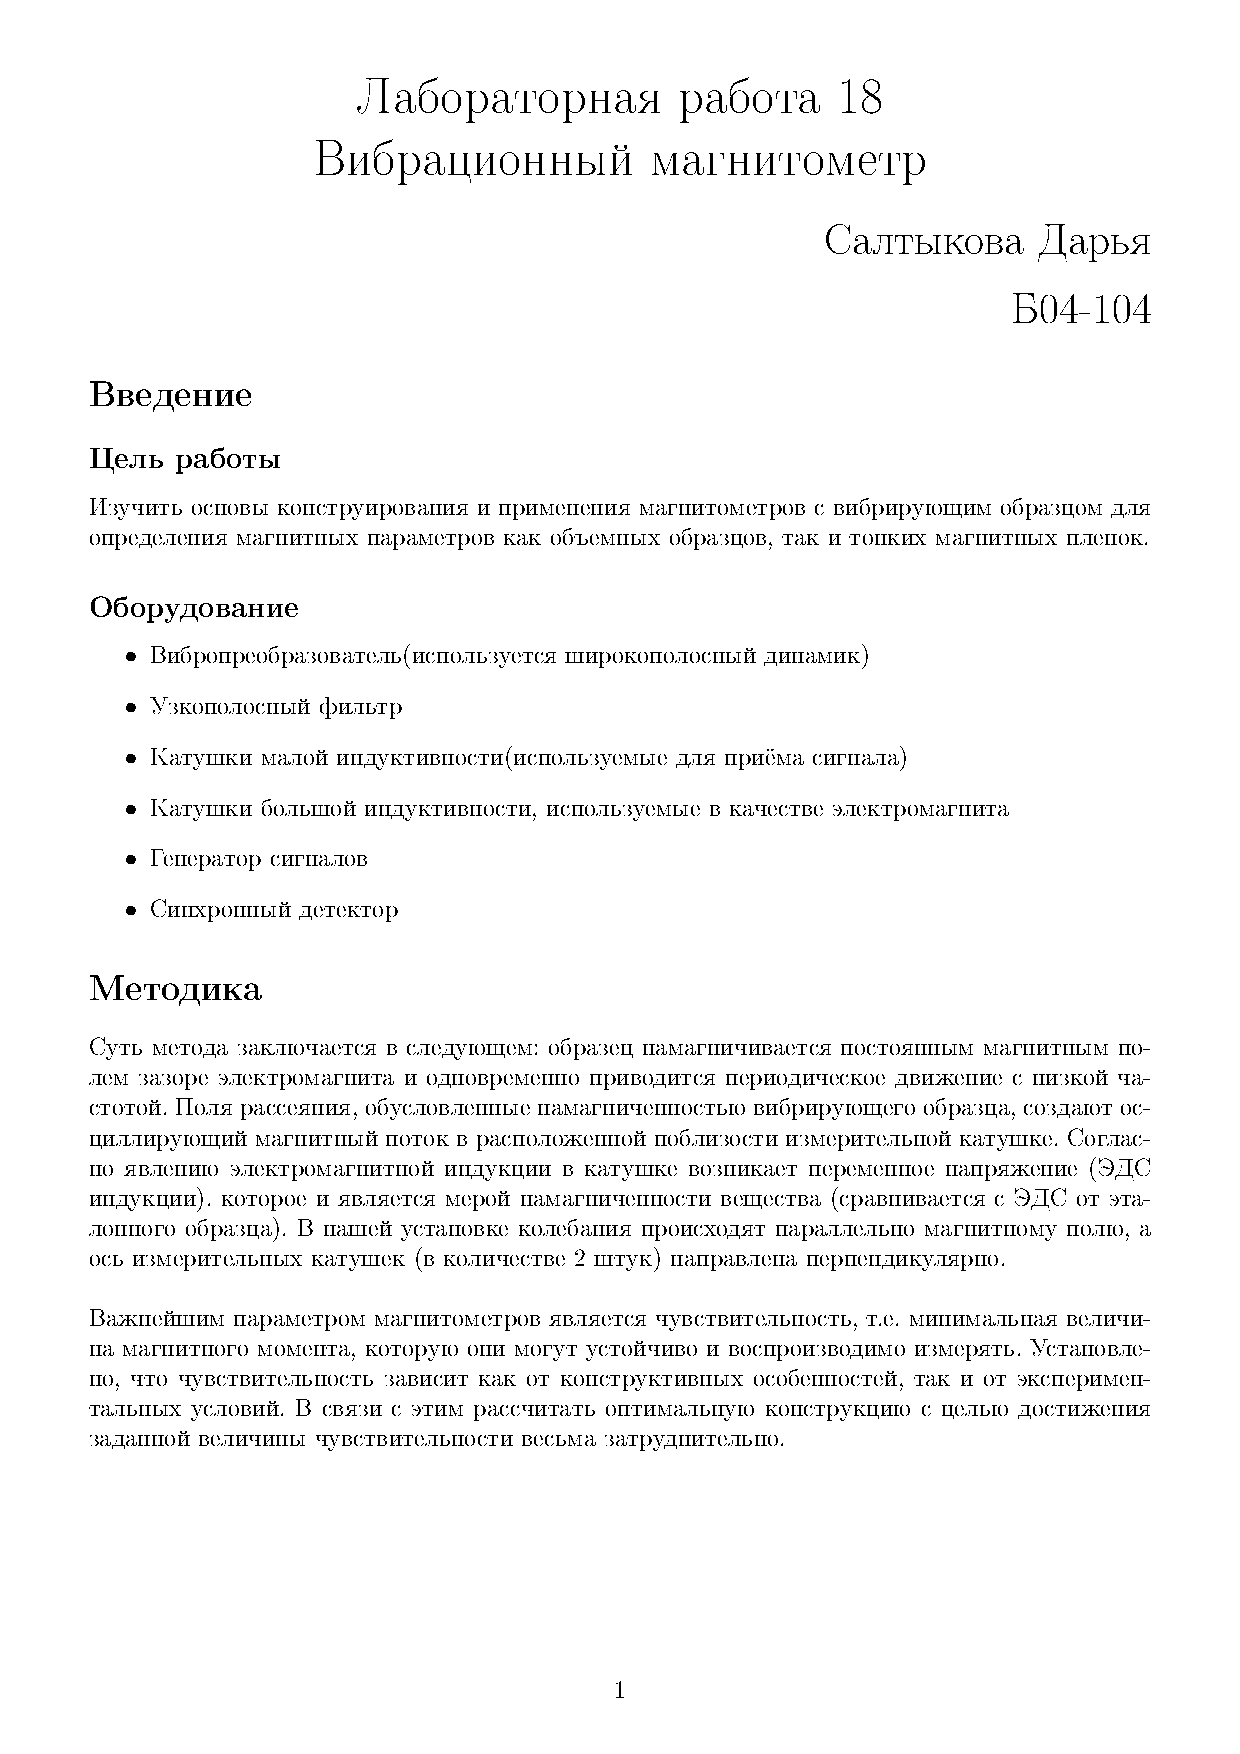
\includegraphics[width = 0.95\linewidth]{main.png}
    \caption{Зависимости интенсивности от мощности}
    \label{fig:intensuty}
\end{figure}

Для нахождения эффективности акустооптической ячейки рассмотрим измерения из таблиц 3 и 4, проведённые при одинаковой силе тока. 
Нанесём на график зависимость отношения интенсивности дифрагированного света к интенсивности падающего света от мощности.

Как видно на рисунке \ref{fig:eff}, отношение $I_{1} / I_{0}$ меняется в зависимости от мощности. То есть коэффициент дифракционной интенсивности различный для разных мощностей. 

Энергетическая эффективность ячейки есть коэффициент наклона изображенной на рисунке \ref{fig:eff} зависимости. Таким образом:
$$
\eta_{\text{энерг}} = 0.62 \pm 0.15 \frac{1}{\text{мкВт}}
$$

\begin{figure}[htbp]
    \centering
    \includegraphics[width = 0.95 \linewidth]{eff.png}
    \caption{Зависимость отношения $I_{1} / I_0$ от мощности}
    \label{fig:eff}
\end{figure}

\section*{\textcolor{header}{Вывод}}
Удалось рассчитать основные характеристики акустооптической ячейки, а именно:
\begin{itemize}
    \item скорость звука в кристалле
    \item Энергетическую эффективность
\end{itemize}





\end{document}
